\documentclass[class=ctexart,crop=false]{standalone}

\usepackage{amsmath,amssymb,enumitem,empheq,tkz-euclide,
diagbox,wrapfig,pgfplots}
\pgfplotsset{compat=newest}
\renewcommand\parallel{\mathrel{/\mskip-2.5mu/}}

\newcommand\px{\mathrel{/\mkern-5mu/}}  %平行
\newcommand\pxeq{\mathrel{\vcenter{     %平行且等于
\ialign{\hfil##\hfil\crcr
$\scriptstyle\px\!$\crcr
\noalign{\nointerlineskip\vskip1pt}$=$\crcr}}}}

%\setCJKmainfont{SimSun}       %设置西文字体为times new roman
%\setCJKsansfont{SimSun}             %设置中文字体为宋体
%\setCJKmonofont{STKaiti}
%\setsansfont{TeX Gyre Termes}            %设置typewriter family中文字体为楷体
%\setmonofont{TeX Gyre Termes}

\usetikzlibrary{calc,intersections,through,backgrounds,patterns}
\newcounter{para}
\newcommand\mypara{\par\refstepcounter{para}\thepara.\space}%设置typewriter family西文字体为times new roman
\newcommand*\circled[1]{\tikz[baseline=(char.base)]{
            \node[shape=circle,draw,inner sep=1.3pt] (char) {#1};}}
\begin{document}
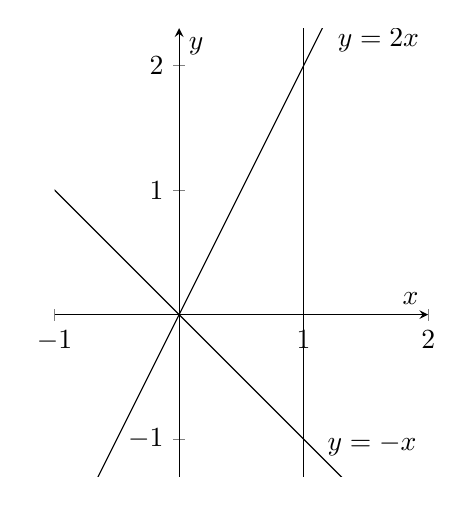
\begin{tikzpicture}
    \begin{axis}[      
        unit vector ratio*=1 1 1 ,
        axis x line = middle,
        axis y line = middle,
        xlabel      = {$x$},
        ylabel      = {$y$},
        xmin=-1, xmax=2,
        ymin=-1.3, ymax=2.3,
        legend pos=outer north east,
        legend style={draw=none},]
        \addplot[black,samples=100] {-x};  
        \addplot[black,samples=100] {2*x};
        \addplot[black,samples=100] (1,x);
        \node at (1.6,2.2) {$y=2x$};
        \node at (1.55,-1.05) {$y=-x$};
    \end{axis}
\end{tikzpicture}\\
$z=3x+2y\Leftrightarrow y=\frac{1}{2}(-3x+z)$\\
则截距越大,$z$越大\\
显然,选取点 $(1,2)z=3+2\times 2=7$最大
\end{document}